% !TeX spellcheck = en_US
\section{Problem 5}

The given neural network consists of two layers and three neurons. On the first one, activation function is \verb*|logsig| or \verb*|swish| and on the second one is \verb*|purelin|. On the left side of figure~\ref{fig:prob_5_responses} we see the sketches for all outputs when the activation function is \verb*|logsig| and on the right side all outputs with activation function being \verb*|swish|.

\begin{figure}[H]
	\centering
	\begin{subfigure}{0.47\textwidth}
		\centering
		\caption{}
		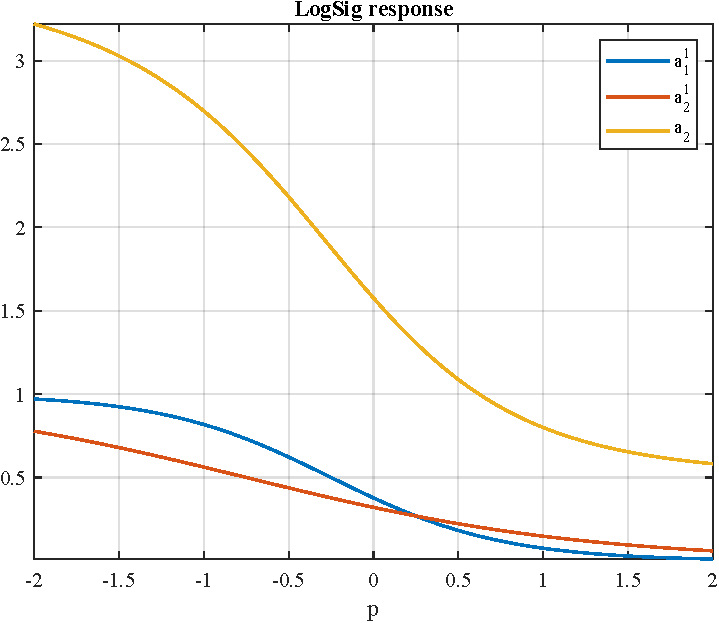
\includegraphics[width=\textwidth]{../Problem 5/logsig_activation.pdf}
	\end{subfigure}
	\hspace{1mm}
	\begin{subfigure}{0.47\textwidth}
		\centering
		\caption{}
		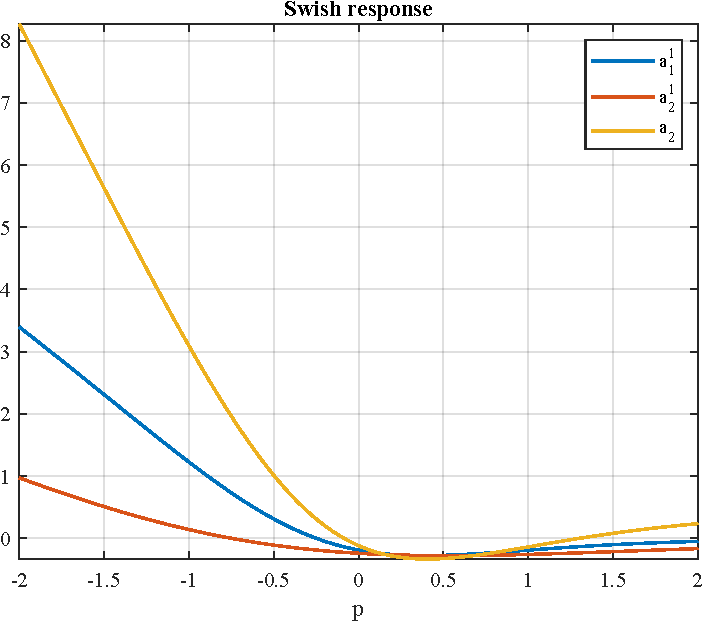
\includegraphics[width=\textwidth]{../Problem 5/swish_activation.pdf}
	\end{subfigure}
	\caption{Responses of different outputs of the neural network}
	\label{fig:prob_5_responses}
\end{figure}